\documentclass{article}
\usepackage[russian]{babel}
\usepackage[utf8]{inputenc}
\usepackage{amsfonts}
\usepackage{amssymb}
\usepackage{listings}
\usepackage{amsmath}
\usepackage{amsthm}
\usepackage{minted}
\usepackage{indentfirst}
\usepackage{hyperref}
\usepackage{cleveref}
\usepackage{graphicx}
\usepackage{wrapfig}
\usepackage{tikz}
\usepackage{ragged2e}
\usepackage{multirow}
\usepackage{subfig}

\title{СМВМ, задание №3}
\author{Болохонов Артем Владимирович}

\begin{document}

\date{}
\maketitle

\textbf{Описание задания:} решалась задача об изгибе балки распределенной нагрузкой. Программа решалась на языке программирования \textit{Python}.


Расчеты проводились на компьютере AMD Ryzen 7 7700x 4.5GHz (up to 5.4 GHz), 8 cores; DIMM DDR5 32 Gb 6000 MHz.


\begin{table}[H]
\centering
\begin{tabular}{|c|l|l|l|l|l|l|}
\hline
N   & $||E_r||_\infty$ & R        & $||E_r||_{L_2}$ & R        & $\mu([K])$ & t (sec) \\ \hline
2   & 3.18e-01       & ------        & 3.43e-01      & ------        & 3.19 & 0.0       \\ \hline
4   & 1.13e-01       & 1.49 & 1.00e-01      & 1.78 & 1.20e+01 & 0.0       \\ \hline
8   & 3.11e-02       & 1.86 & 2.60e-02      & 1.95 & 3.98e+01 & 0.0       \\ \hline
16  & 7.97e-03       & 1.97 & 6.56e-03      & 1.99 & 1.34e+02 & 1.0014e-03       \\ \hline
32  & 2.00e-03       & 1.99 & 1.64e-03      & 2.00 & 4.78e+02 & 1.9999e-03       \\ \hline
64  & 5.01e-04       & 2.00 & 4.10e-04      & 2.00 & 1.79e+03 & 3.0007e-03       \\ \hline
128 & 1.24e-04       & 2.01 & 1.01e-04      & 2.02 & 6.90e+03 & 4.0007e-03       \\ \hline
\end{tabular}
\caption{результаты численных экспериментов}
\end{table}


\begin{figure}[H]
  \centering
  \subfloat{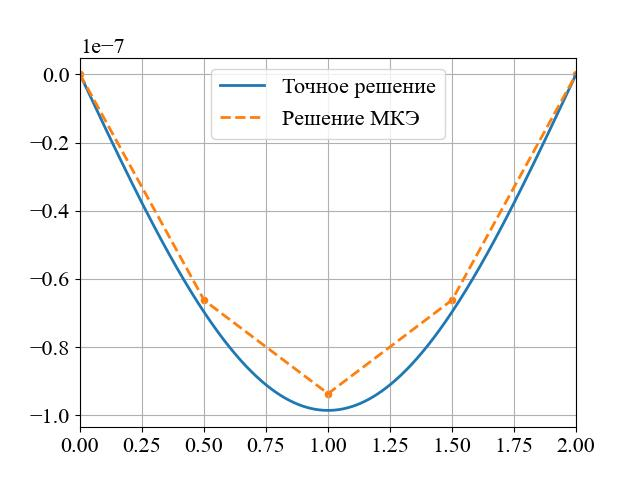
\includegraphics[width=0.5\textwidth]{4.jpeg}}
  \hfill
  \subfloat{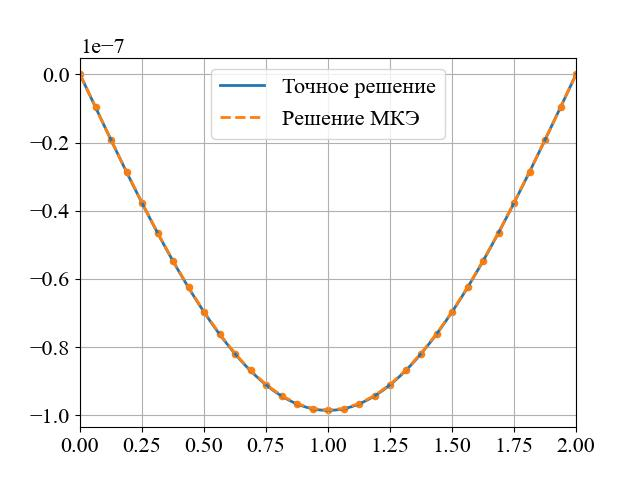
\includegraphics[width=0.5\textwidth]{32.jpeg}}
  \caption{\centeringсравнение точного и приближенного решения на сетке с разбиением на 4 и 32 ячейки}
\end{figure}

Ответы на вопросы:
\begin{enumerate}
    \item \textit{Результаты численных экспериментов} \\
    Учитывая, что матрица получилась трехдиагональная, то суммарная сложность получится $\operatorname{O}(n)$.
    \item \textit{Влияет ли способ нумерации элементов на вычислительную эффективность алгоритма?} \\
    Да, влияет. В данном случае именно из-за нумерации элементов мы получили трехдиагональную матрицу, следственно и уменьшили сложность алгоритма.
    \item \textit{Оцените, во сколько раз увеличится глобальная СЛАУ, если вместо n линейных элементов использовать n квадратичных.} \\
    Размер глобальной СЛАУ должен увеличиться приблизительно в два раза, до $\left( (2n + 1), (2n + 1)\right)$.
    \item \textit{Каким образом найти локальную матрицу жесткости и вектор правой части, если нет возможности провести интегрирование аналитически?} \\
    Для подобного случая можно использовать методы численного интегрирования, такие как метод трапеций, Симпсона или сплайнов.
\end{enumerate}
\end{document}
